% !Mode:: "TeX:UTF-8"

\chapter{}
\textbf{
Recall the problem of finding the number of inversions. As in the text, we are given a sequence of $n$ numbers $a_1,...,a_n$, which we assume are all distinct, and we define an inversion to be a pair $i<j$ such that $a_i>a_j$.
}

\textbf{
We motivated the problem of counting inversions as a good measure of how different two ordering are. However, one might feel that this measure is too sensitive. Let's call a pair a \emph{significant inversion} if $i<j$ and $a_i>2a_j$. Give an $O(n log n)$ algorithm to count the number of significant inversions between two orderings.
}
\hspace*{\fill} \\

It's similar as the algorithm of finding the number of inversions expect that we need two pointers in the left array, which point to the current element of the left array and the least number that greater than twice of the current element of the right array. Consider the following example show in figure~\ref{fig1}. There are two arrays, they are array $A$ and array $B$. Suppose Both of the two arrays have been sorted and counted about the inversion number satisfying $i<j$ and $a_i>a_j$(we call this \emph{twice inversion}), we now need to merge $A$ and $B$ as well as count the twice inversion between $A$ and $B$.
\\
\begin{figure}[!htbp]
\centering
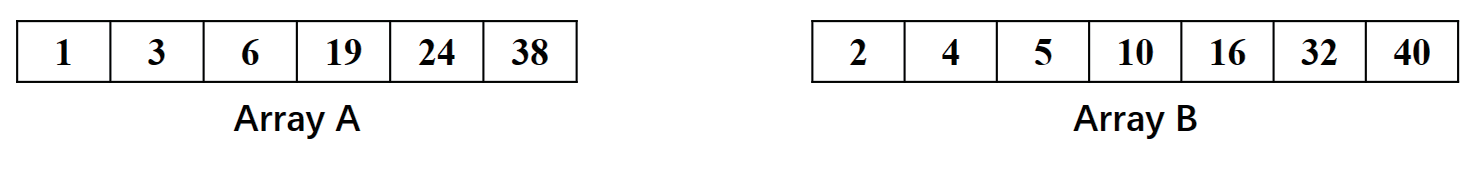
\includegraphics[width=0.8\textwidth]{figures/1.eps}
\caption{Two subarrays}\label{fig1}
\end{figure}

As is showed in figure~\ref{fig2}, we construct merge array which is initialized as null. And we set three pointers $i,j,k$. Pointer $i$ and pointer $j$ point the current element in array $A$ and array $B$, respectively. Pointer $k$ points to the element in $A$ which is the least number greater the the current element in array $B$.
\\
\begin{figure}[!htbp]
\centering
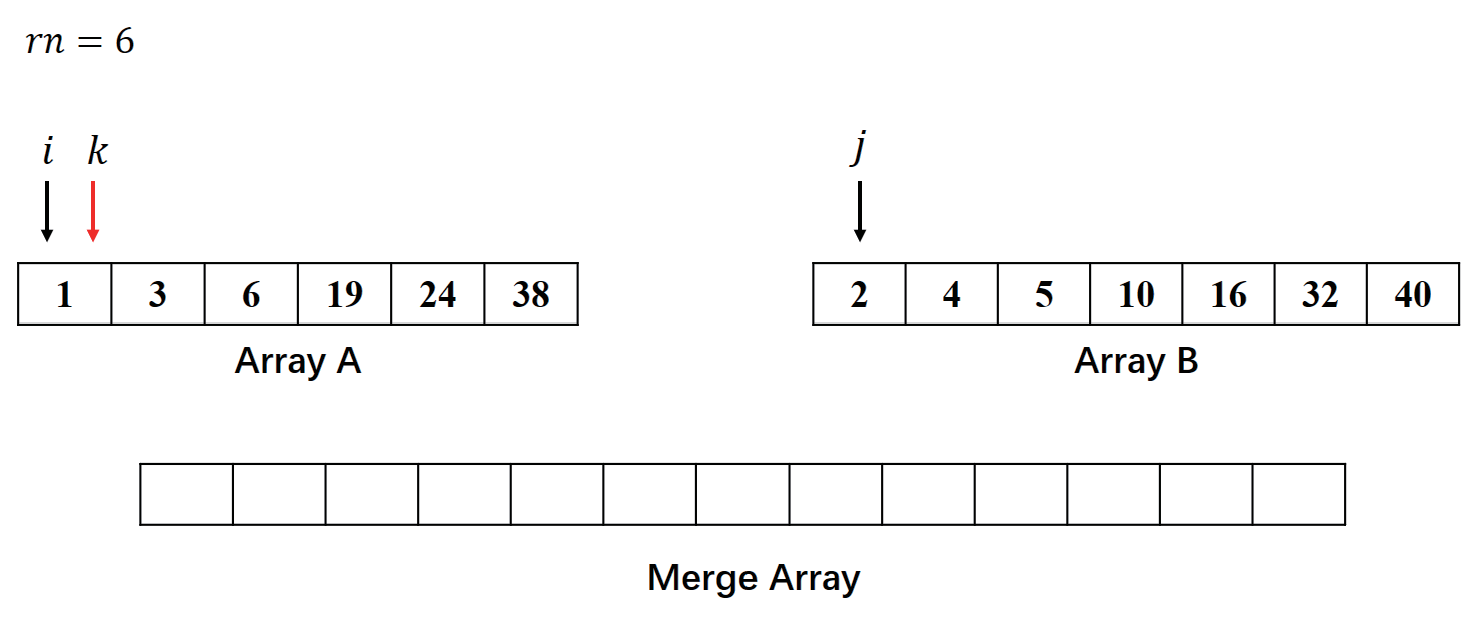
\includegraphics[width=0.8\textwidth]{figures/2.eps}
\caption{Two subarrays}\label{fig2}
\end{figure}

We compare each current element in $A$ and $B$. If $A[i] < B[j]$, then we add $A[i]$ to the merge array, and move forward pointer $i$ by 1 step. Besides we need to keep pointer $k$ not behind pointer $i$. If $A[i] > B[j]$, we need to find the least element $A[k]$ in $A$, which is greater than double of $A[j]$. We set the current twice inversion number $rn$ as $len(A)-k+1$, and add the current twice inversion number to the result. Figure~\ref{fig3} shows one state of the middle progress. And Figure~\ref{fig4} shows the final state.
\\
\begin{figure}[!htbp]
\centering
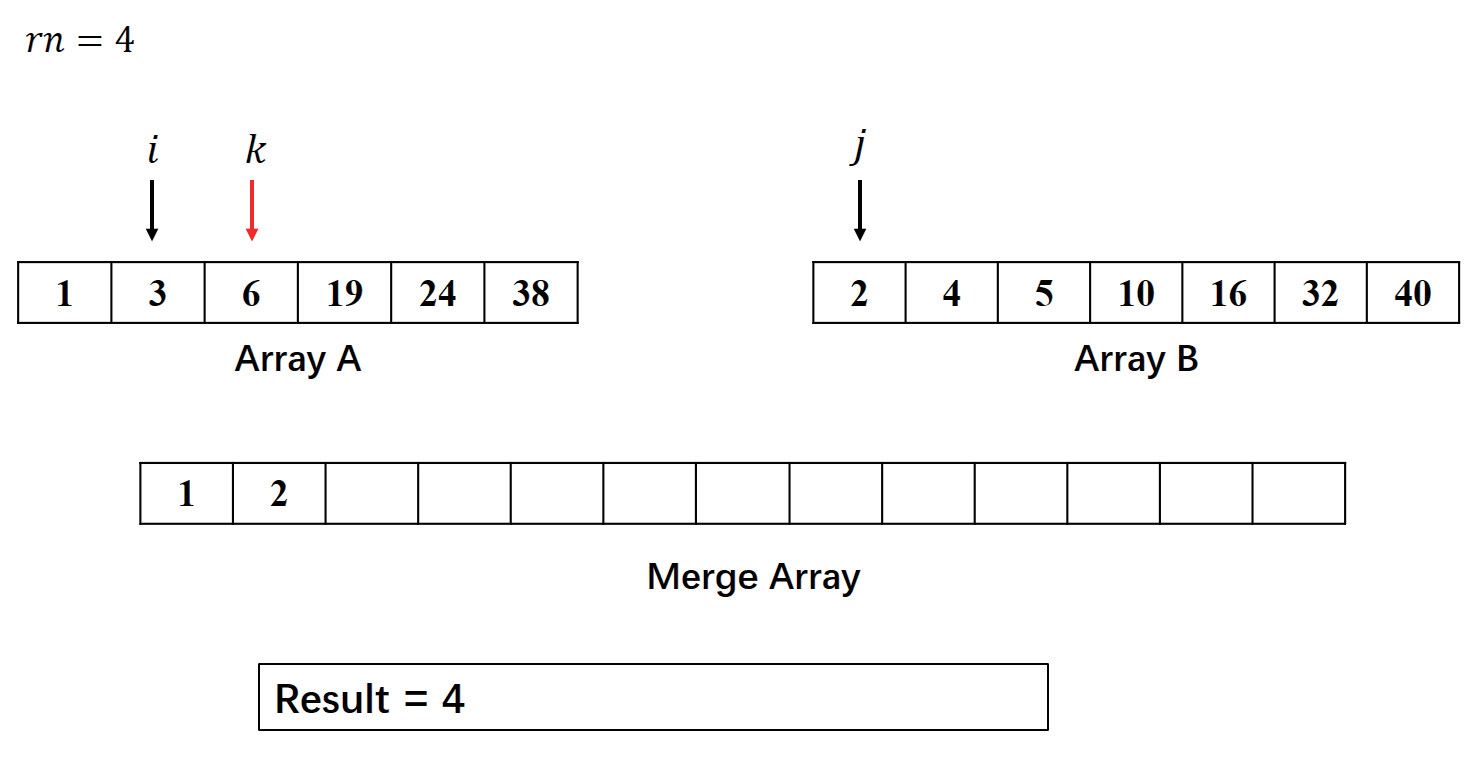
\includegraphics[width=0.8\textwidth]{figures/3.eps}
\caption{Two subarrays}\label{fig3}
\end{figure}
\\
\begin{figure}[!htbp]
\centering
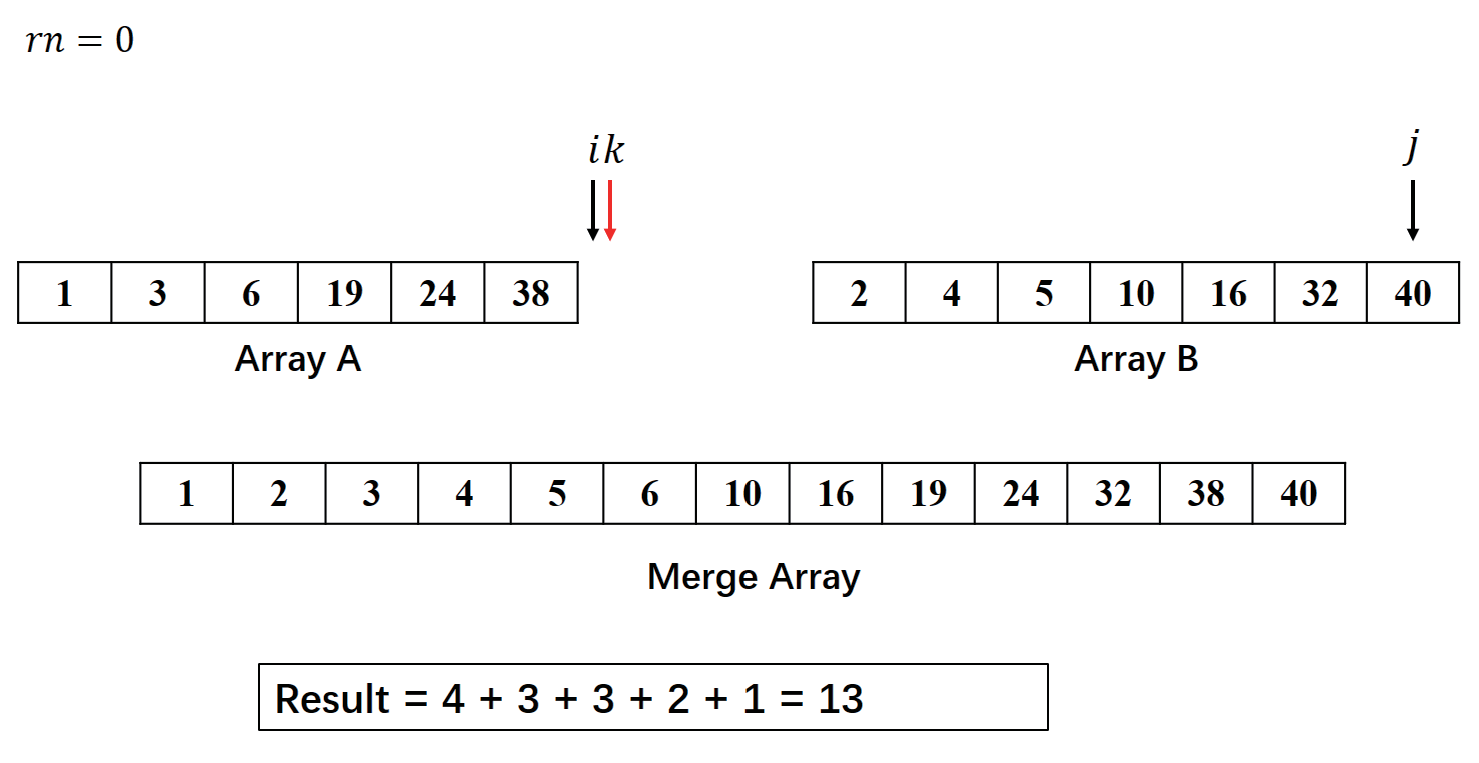
\includegraphics[width=0.8\textwidth]{figures/4.eps}
\caption{Two subarrays}\label{fig4}
\end{figure}

Next, we give the merge part algorithm in Alg~\ref{CTIN}.
\begin{algorithm}
\caption{Count twice inversion number}
\label{CTIN}
\begin{algorithmic}[1]
\REQUIRE Array $A$ and $B$
\STATE Result = 0
\STATE MergeArray = $\phi$
\WHILE{$i<length(A)$ and $j<lengthB$}
    \IF{$A[i]<B[j]$}
        \STATE{Add $A[i]$ to MergeArray}
        \STATE{$i++$}
        \IF{$k<i$}
            \STATE{$k=i$}
            \STATE{$rn--$}
        \ENDIF
    \ELSE
        \WHILE{$k<length(A)$ and $A[k]<=2B[j]$}
            \STATE{$k++$}
            \STATE{$rn--$}
        \ENDWHILE
        \STATE{Add $B[j]$ to merge array}
        \STATE{Add rn to the result}
        \STATE{$j$++}
    \ENDIF
\ENDWHILE
\STATE{Add the remain elements in $A$ or $B$ to merge result}
\STATE Return sorted result
\end{algorithmic}
\end{algorithm}